\documentclass[tikz]{standalone}

\usetikzlibrary{positioning, backgrounds,patterns,fadings}

\usepackage{lmodern}
\usepackage{microtype}

\begin{tikzfadingfrompicture}[name=myfading]
\node[text=transparent!10]
{\fontsize{60}{60}\selectfont \textbf{8}};
\end{tikzfadingfrompicture}

\newcommand{\tile}[2]{
    \begin{tikzpicture}[background rectangle/.style={fill=olive!15}, show background rectangle, inner sep=0pt]
    \node[minimum width=2.5cm,minimum height=3cm] at (0,1) {
    \fontsize{60}{60}\selectfont \textbf{\textcolor{#2}{#1}}
    };
%     \node[circle,line width=2pt,fill=olive!20,draw=olive!22,minimum size = 30] at (0,-.8){}; 
    \shade[ball color=olive!10] (0,-.65) circle (.5);
    \end{tikzpicture}
}


\begin{document}

\tile{8}{blue}\begin{tikzpicture}[background rectangle/.style={fill=olive!15}, show background rectangle, inner sep=0pt]
\fill[path fading=myfading, shading angle=50,  ball color=blue!80] (-1.25cm,-1.5cm) rectangle (1.25cm,1.5cm);
\end{tikzpicture}

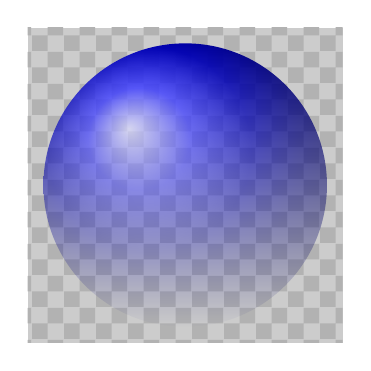
\begin{tikzpicture}
% Checker board
\fill [black!20] (0,0) rectangle (4,4);
\path [pattern=checkerboard,pattern color=black!30] (0,0) rectangle (4,4);
\shade [ball color=blue,path fading=south] (2,2) circle (1.8);
\end{tikzpicture}


\begin{tikzpicture}
\shade [ball color=olive!15,path fading=north] (-1.25,-2) rectangle (1.25,2);
\end{tikzpicture}


% \tile{8}{blue}
% \begin{tikzpicture}
% \definecolor{amber2}{RGB}{239, 215, 74}
% \fill[orange] (0,0) circle[radius=1];
% \fill[path fading=myfading, ball color=amber2, shading angle=300] (0,0) circle[radius=1];
% \end{tikzpicture}

\end{document}
